\chapter{General Introduction}
\section{Introduction}
Particle Physics or sometimes called High Energy Physics, is the field of physics that pursues the ultimate structure of matter, this is possible in two ways, one is to look for elementary particles, the ultimate constituents of matter at their smallest scale and the other is to clarify what interactions are acting among them
 \emph{(forces)} to construct matter as we see it.

In our current view, all matter is made of three kind of elementary particles, \emph{leptons}, \emph{quarks} and \emph{mediators}.

Leptons have spin $\frac{1}{2}$, they naturally fall into three families, these are electron, muon, tau and their associated neutral neutrinos, those are described by lepton numbers for the example the electron has electron number 1 and the muon has electron number 0 and muon number 1 and so on. The three charged leptons have electric  charge -1. There are also six anti leptons for example the positron which has electron number of -1 and electric charge +1, so all in all we have 12 leptons.

The quarks have spin $\frac{1}{2}$ too, there are six flavours of quarks, up, down, top, bottom, charm and strange, quarks have a colour charge, which is property that is related to the strong interactions,  as the leptons there are also six anti quarks, we will talk about them in more details in following sections. 

Every interaction has its mediators, the photon for electromagnetic interactions, the gluon for the strong interactions, the two W' and Z for the weak interactions, and presumably the graviton for gravity.            

 
There are four forces in nature, gravity, electromagnetism, weak nuclear force and strong nuclear force. In this essay our work will be on the strong nuclear force. 

\section{Quarks}
Quarks and leptons are the building blocks which build up matter. As mentioned above there are six "flavours" of quarks, these are up, down charm strange, top and bottom.

Quarks can successfully account for all known mesons and baryon which are known as hadrons, which are particles with spin $\frac{1}{2}$. Mesons consist of quark and anti quark for example the positive pion $\pi^+$ which consists of up and anti down quarks. Baryons consist of three quarks or three anti quarks for example the proton which consists of two up quarks and one down quark.


Quarks carry colour quantum number: red, green or blue, the colour name here is an analogy  that is famously used among physicists to describe a three kind of generating force, we may call them by a number or any other index, also we can think of it as a three primary additive colours. Since all hadrons are colour charge neutral or colourless particles they have white charge. 

Unlike other elementary particles quarks carry fractional charge and possess new quantum numbers.
The table \ref{table1.1} summarizes some properties of quarks. Each quark flavour is associated with its own quantum number\footnote{These are the set of numbers that describes a conserved quantities in the dynamic of a quantum system, for example the set of numerical solutions of Schrödinger equation of the Hydrogen atom.}(the capital letters), those quantum numbers describes the decay of the particles, those first were meant to explain the fact that some particles decay slower than other particles, for example the first mentioned below the "Strangeness", it has been noticed that the higher the mass the lower the strangeness,  these numbers are conserved in strong and electromagnetic interactions but not in weak interaction, 
These are: 
\begin{itemize}
\item[•]Strangeness: $S=-1$ for s-quark.

\item[•]Charm: $C=+1$ for c-quark.

\item[•]Beauty: $\tilde{B}=-1$ for b-quark. 

\item[•] t - quark has life time too short to form hadrons. 
\item[•]up and down quarks have nameless flavour quantum numbers.
\end{itemize} \citep{particle}
%\Jnote{What exactly is conserved here? Are these six values or just one?} 

\begin{table}
\begin{center} 
 \begin{tabular}{|c|c|c|c|} \hline 
  Name (Flavour) & Symbol & Electric charge(in units of e) & Mass  \\ \hline 
  $\text{Up}$ & $\text{u}$ &$ +\frac{2}{3}$ & $1.7-3.1 \frac{Mev}{c^2}$\\\hline
  $\text{Down}$&$\text{d}$&$-\frac{1}{3}$& $4.1-5.7\frac{Mev}{c^2}$\\\hline
  $\text{charm}$&$\text{c}$&$+\frac{2}{3}$&$1.18-1.34\frac{Gev}{c^2}$\\\hline
  $\text{strange}$&$\text{s}$&$-\frac{1}{3}$&$80-130\frac{Mev}{c^2}$\\\hline
  $\text{top}$&$\text{t}$&$+\frac{2}{3}$&$172.3-173.5\frac{Gev}{c^2}$\\\hline
  $\text{bottom}$&$\text{b}$&$-\frac{1}{3}$&$4.13-4.37\frac{Gev}{c^2}$\\\hline
 \end{tabular}
\caption{properties of Quarks}
\label{table1.1}
\end{center}
\end{table}

%\Jnote{Maybe extend the table to explain other properties of quarks?}

\Jnote{Citations: If section(s) are based on a textbook, cite it in
  the beginning, saying something like ``the following
  presentation is based on \textbackslash cite\{...\}''}

\section{Strong Force}
As we mentioned the elementary particles that mediate these interactions
%\Jnote{''this interaction'' or ''these interactions''}
are eight called gluons, which come from the gauge group $SU(3)$ which has eight generators, gluons mediate the interaction between quarks.

Gluon is massless spin $1$ particle, carrying charge called colour charges, gluons look like photons but photons do not carry electric charge, because of that gluons can interact among themselves unlike photons.
Normally the range of the force can be calculated by a simple argument of the uncertainty\footnote{$\Delta E \Delta t \approx m c^2 \Delta t > \frac{\hbar}{2} \Longrightarrow range = c \Delta t > \frac{\hbar}{2 m c}$}, but this not the case for the strong force, the strong force is more complicated
and involves a concept known as confinement.

The colour charge has strange property that it exerts a constant force that binds colour carrying particles together, this can be visualized using the analogy of a rubber band, the stronger you pull on the rubber band the tighter it feels.
If we do not pull on it at all, it hangs loose. The same thing happens for the particles,  that means at a very short distance, the force is relaxed and the particles behave as free particles, as the distance between them increases the force acts like a rubber band, the force gets them back in stronger pulling and when the rubber band is stretched beyond its limits then it will cut into many pieces producing more particles. This phenomenon is known as the colour confinement. In other words those particles tend not to be separated by a macroscopic distance.
This limits the range of strong force, which is believed to be on order of $10^{-15}\si{m}$,
the dimension of a nuclear particle.

The theory which describes this force is called $Quantum$ $Chromodynamics$.
\Jnote{Citation for this section would be nice.}

\section{Large Hadron Collider}

Hadron colliders are devices made to explore the world of particle physics, they work as theories testers and also as a discovery machines, an example of these hadron Colliders is the LHC in CERN.

In the Large hadron Collider two beams of hadrons  (protons) are being accelerated to a high kinetic energy and then collided with each other. It has started operation in 2009.
 
Most of the interesting physics at LHC involves investigating the results of these interactions(collisions), as a result of this collision stable partons are formed, partons consists of quarks and qluons. The detectors gather information about the particles, including their speed, mass, charge, from which we can identify the particles. The detectors consists of sub-detectors, each is designed to look for a particular properties. For example, the tracking devices reveal of the particle; calorimeters stop, absorb and the particle energy.   

Because of the complex nature of the event at the hadrons colliders, the description of the final state involves a multi-particle calculations. The accurate prediction of the final state in hadron colliders is still one the hardest problems, this problem roots to the non-abelian nature of QCD, which leads to a colour confinement at a long distances. The two main problems are the description of the hadron formation and the evolution of QCD final states from short to long distances. Those problems can be tackled to a good approximation by Monte-Carlo event generators.


     
      
\section{Monte Carlo Method}
The name Monte Carlo method is set of mathematical tools that first used by scientist working on the nuclear project in Los Alamos. The essence of the is to generate numbers with probability that can be used to study physical phenomena. In our context the definition of Monte Carlo method would be, that in which we use randomly generated numbers to imitate a physical behaviour that is not necessarily considered to be random \citep{montecarlo}.

\subsection{Pseudo-random numbers}
In a computer these are generated using a deterministic algorithm that generates a set of numbers that exhibits statistical randomness, those numbers are called pseudo-random \citep{montecarlo}.


\subsection{Samples with different PDFs}

Generating samples of different probability distribution function(pdf) is essential since we are simulating various variables that have different numerical behaviour. For example if our pseudo-random numbers are uniformly\footnote{Uniform means that every value in the range of the distribution is equally likely to occur. This distribution is widely used for generating random numbers for other distributions, it is denoted by $U$.} distributed in the interval $[0,1]$  and instead we need numbers that have normal distribution restricted to the same interval. I will discuss two methods, which are used in this essay.

\subsection{The acceptance-rejection method}

The acceptance-rejection method was developed by von Neumann \citep{Weinzierl}.
Assume we have access to a sample which is distributed according to the pdf $f(x)$,
and the let us denote the pdf of the required distribution by $p(x)$, we assume that for both $p(x)$ and $f(x)$ $x$ varies over a finite interval.
 
In simple words, first we generate $x$ according to the uniform distribution over a given interval assume $[0,1]$ 
, then we find the maximum of $f(x)$, and then calculates $p(x)$, then we generate another number $y$ which is also uniformly distributed over the interval $[0,f_{max}(x)]$, and checks  $y \times f(x) \leq p(x)$.
If this the case then accept $x$, if not reject $x$ and start again, example of that, if have a number $x$ that is fall under uniform distribution and we want to reshape this so that we get a number  that has the distribution $\frac{1}{x}$, then we find the maximum value of probability density function ($p(x)$) for $x$, here we add small number to $x$ so that we avoid the singular point when $x = 0$, after that we generate another sample $y$ that is also uniformly distributed in the interval $[0,pdf_{max}]$, 
now we check if $y $ is less than $p(x)$ we add $x$ to our distribution if not we start again. The histograms in figure \ref{fig:2} demonstrate the example above.   

\begin{figure}[hbtp]
\centering
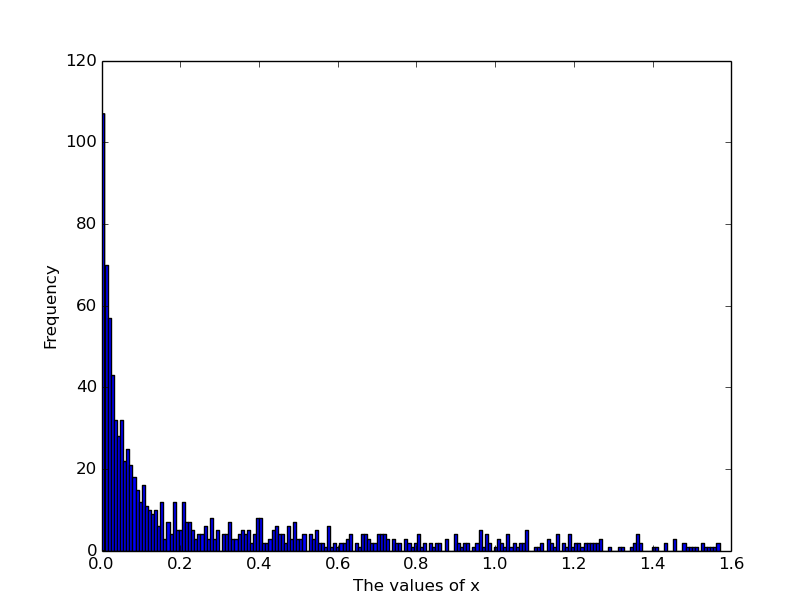
\includegraphics[scale=.5]{images/inverse_method.png}
\caption{Generating values with distribution $\frac{1}{x}$}\label{fig:2}
\end{figure}

%\begin{figure}
%    \centering
%    \begin{subfigure}[b]{0.5\textwidth}
%        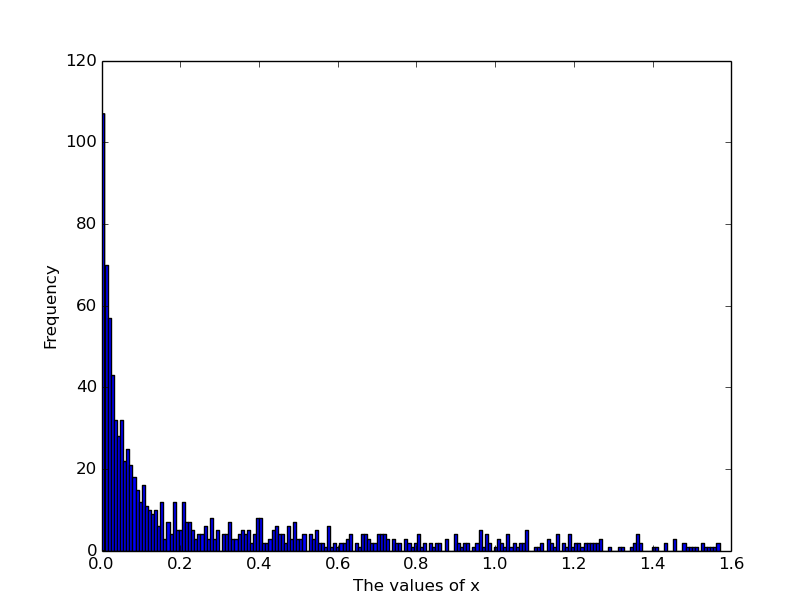
\includegraphics[width=\textwidth]{images/inverse_method.png}
%        \caption{Theta values}
%        \label{fig2}
%    \end{subfigure}
%    ~ %add desired spacing between images, e. g. ~, \quad, \qquad, \hfill etc. 
%      %(or a blank line to force the subfigure onto a new line)
%    \begin{subfigure}[b]{0.5\textwidth}
%        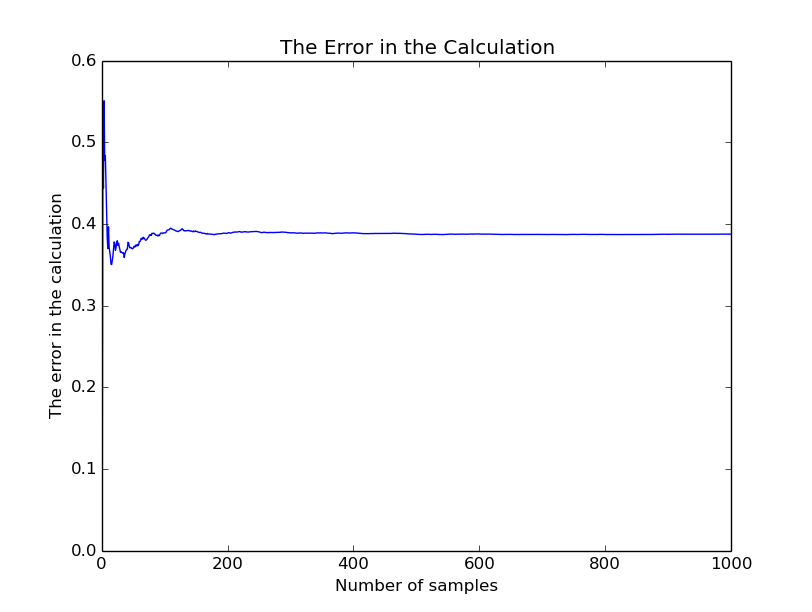
\includegraphics[width=\textwidth]{images/uncertainity_.png}
%        \caption{The uncertainty}
%        \label{fig2}
%    \end{subfigure}
%    \label{Fig:2}
%\caption{}
%\end{figure}

Another related example of this method is calculation of pi, assume we have a box of side length D and a circle of diameter D inside that box, now the probability that a point in the box and is also in the circle is approximately the area of the circle over the area of the box, which is $\pi$ over 4 here, hence, from this we can approximate the value of $\pi$. The histograms in Figure \ref{fig:1.1} exhibits this calculation and also the error in the calculation\citep{Weinzierl}.


\begin{figure}
    \centering
    \begin{subfigure}[b]{0.5\textwidth}
        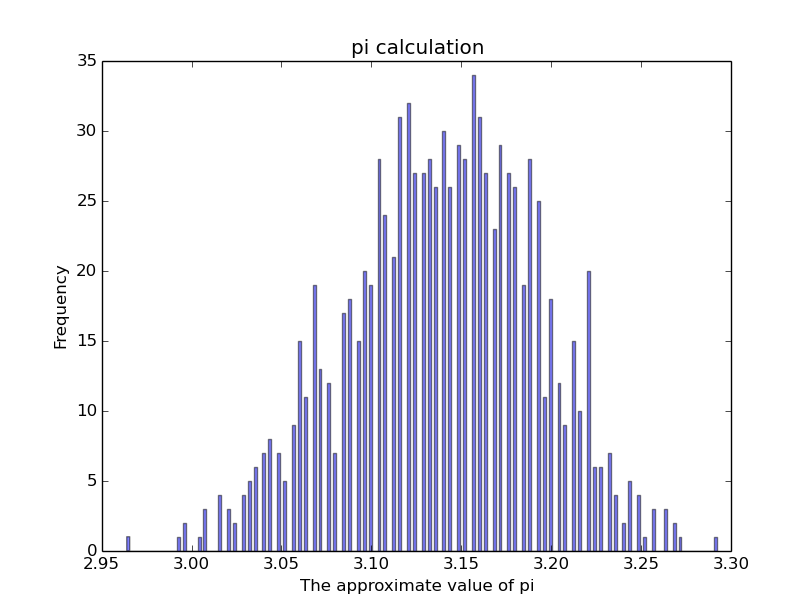
\includegraphics[scale=.5]{images/pi_value.png} 
        \caption{pi value}
        \label{fig:gull}
    \end{subfigure}
    ~ %add desired spacing between images, e. g. ~, \quad, \qquad, \hfill etc. 
      %(or a blank line to force the subfigure onto a new line)
    \begin{subfigure}[b]{0.5\textwidth}
        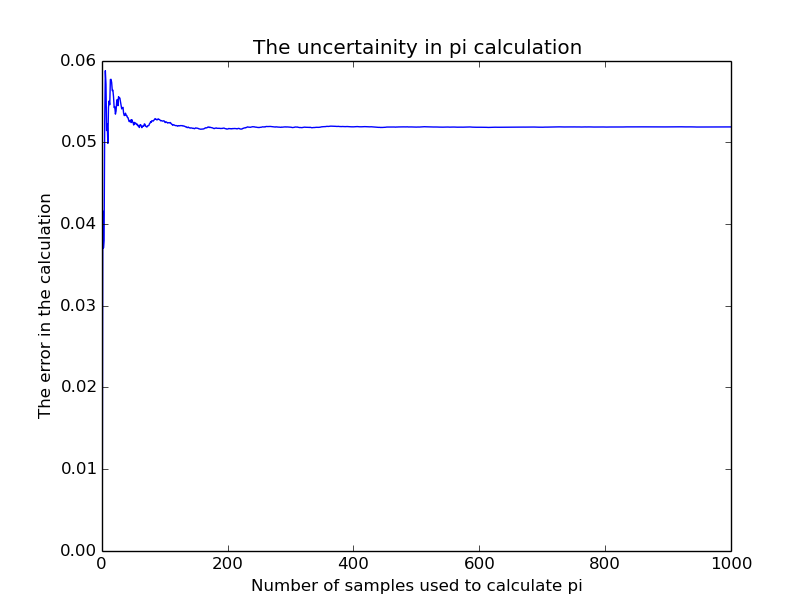
\includegraphics[scale=0.5]{images/uncertainity_pi.png}
        \caption{The uncertainty}
        \label{fig:tiger}
    \end{subfigure}
    \label{Fig:1}
\caption{At the top, this a histogram shows the values of $\pi$ that are generated from sampling 1000 numbers. At the bottom the plot shows the error in the calculation when we use different number of samples} 
\label{fig:1.1}
\end{figure}

%\Jnote{Consider giving a file name (files will be attached as appendix)
%whenever you are presenting a calculation, like with the histograms here.}


\subsection{The module random in python}

The samples above were generated using Python module \verb+random+, here are few words about this module.

%\Jnote{For module, variable and file names you can use verbatim command like this:
%\textbackslash verb+my\_file.py+}.
 
This module implements pseudo-random number generators for various distributions.

In a computer pseudo-random numbers are generated using a deterministic algorithm that generates a set of numbers that exhibits statistical randomness, those numbers are called pseudo-random.

For integers, there is uniform selection from a range. For sequences, there is uniform selection of a random element, a function to generate a random permutation of a list in-place, and a function for random sampling without replacement.

On the real line, there are functions to compute uniform, normal (Gaussian), lognormal, negative exponential, gamma, and beta distributions. For generating distributions of angles, the von Mises distribution is available.

Almost all module functions depend on the basic function random(), which generates a random float uniformly in the semi-open range $[0.0, 1.0)$. Python uses the Mersenne Twister as the core generator. It produces 53-bit precision floats and has a period of $2^{19937}-1$\citep{python}.
